\documentclass[reqno]{amsart}
\usepackage{amscd, amssymb, amsmath, amsthm}
\usepackage{graphicx}
\usepackage[colorlinks=true,linkcolor=blue]{hyperref}
\usepackage[utf8]{inputenc}
\usepackage[T1]{fontenc}
\usepackage{textcomp}
\usepackage{babel}
%% for identity function 1:
\usepackage{bbm}
%%For category theory diagrams:
\usepackage{tikz-cd}

%\usepackage[backend=biber]{biblatex}
%\addbibresource{.bib}


\setlength\parindent{0pt}

\pdfsuppresswarningpagegroup=1

\newtheorem{theorem}{Theorem}[section]
\newtheorem{lemma}[theorem]{Lemma}
\newtheorem{proposition}[theorem]{Proposition}
\newtheorem{corollary}[theorem]{Corollary}
\newtheorem{conjecture}[theorem]{Conjecture}

\theoremstyle{definition}
\newtheorem{definition}[theorem]{Definition}
\newtheorem{example}[theorem]{Example}
\newtheorem{exercise}[theorem]{Exercise}
\newtheorem{problem}[theorem]{Problem}
\newtheorem{question}[theorem]{Question}

\theoremstyle{remark}
\newtheorem*{remark}{Remark}
\newtheorem*{note}{Note}
\newtheorem*{solution}{Solution}



%Inequalities
\newcommand{\cycsum}{\sum_{\mathrm{cyc}}}
\newcommand{\symsum}{\sum_{\mathrm{sym}}}
\newcommand{\cycprod}{\prod_{\mathrm{cyc}}}
\newcommand{\symprod}{\prod_{\mathrm{sym}}}

%Linear Algebra

\DeclareMathOperator{\Span}{span}
\DeclareMathOperator{\im}{im}
\DeclareMathOperator{\diag}{diag}
\DeclareMathOperator{\Ker}{Ker}
\DeclareMathOperator{\ob}{ob}
\DeclareMathOperator{\Hom}{Hom}
\DeclareMathOperator{\Mor}{Mor}
\DeclareMathOperator{\sk}{sk}
\DeclareMathOperator{\Vect}{Vect}
\DeclareMathOperator{\Set}{Set}
\DeclareMathOperator{\Group}{Group}
\DeclareMathOperator{\Ring}{Ring}
\DeclareMathOperator{\Ab}{Ab}
\DeclareMathOperator{\Top}{Top}
\DeclareMathOperator{\hTop}{hTop}
\DeclareMathOperator{\Htpy}{Htpy}
\DeclareMathOperator{\Cat}{Cat}
\DeclareMathOperator{\CAT}{CAT}
\DeclareMathOperator{\Cone}{Cone}
\DeclareMathOperator{\dom}{dom}
\DeclareMathOperator{\cod}{cod}
\DeclareMathOperator{\Aut}{Aut}
\DeclareMathOperator{\Mat}{Mat}
\DeclareMathOperator{\Fin}{Fin}
\DeclareMathOperator{\rel}{rel}
\DeclareMathOperator{\Int}{Int}
\DeclareMathOperator{\sgn}{sgn}
\DeclareMathOperator{\Homeo}{Homeo}
\DeclareMathOperator{\SHomeo}{SHomeo}
\DeclareMathOperator{\PSL}{PSL}
\DeclareMathOperator{\Bil}{Bil}
\DeclareMathOperator{\Sym}{Sym}
\DeclareMathOperator{\Skew}{Skew}
\DeclareMathOperator{\Alt}{Alt}
\DeclareMathOperator{\Quad}{Quad}
\DeclareMathOperator{\Sin}{Sin}
\DeclareMathOperator{\Supp}{Supp}
\DeclareMathOperator{\Char}{char}
\DeclareMathOperator{\Teich}{Teich}
\DeclareMathOperator{\GL}{GL}
\DeclareMathOperator{\tr}{tr}
\DeclareMathOperator{\codim}{codim}
\DeclareMathOperator{\coker}{coker}
\DeclareMathOperator{\corank}{corank}
\DeclareMathOperator{\rank}{rank}
\DeclareMathOperator{\Diff}{Diff}
\DeclareMathOperator{\Bun}{Bun}
\DeclareMathOperator{\Sm}{Sm}
\DeclareMathOperator{\Fr}{Fr}
\DeclareMathOperator{\Cob}{Cob}
\DeclareMathOperator{\Ext}{Ext}
\DeclareMathOperator{\Tor}{Tor}



%Row operations
\newcommand{\elem}[1]{% elementary operations
\xrightarrow{\substack{#1}}%
}

\newcommand{\lelem}[1]{% elementary operations (left alignment)
\xrightarrow{\begin{subarray}{l}#1\end{subarray}}%
}

%SS
\DeclareMathOperator{\supp}{supp}
\DeclareMathOperator{\Var}{Var}

%NT
\DeclareMathOperator{\ord}{ord}

%Alg
\DeclareMathOperator{\Rad}{Rad}
\DeclareMathOperator{\Jac}{Jac}

%Misc
\newcommand{\SL}{{\mathrm{SL}}}
\newcommand{\mobgp}{{\mathrm{PSL}_2(\mathbb{C})}}
\newcommand{\id}{{\mathrm{id}}}
\newcommand{\MCG}{{\mathrm{MCG}}}
\newcommand{\PMCG}{{\mathrm{PMCG}}}
\newcommand{\SMCG}{{\mathrm{SMCG}}}
\newcommand{\ud}{{\mathrm{d}}}
\newcommand{\Vol}{{\mathrm{Vol}}}
\newcommand{\Area}{{\mathrm{Area}}}
\newcommand{\diam}{{\mathrm{diam}}}
\newcommand{\End}{{\mathrm{End}}}


\newcommand{\reg}{{\mathtt{reg}}}
\newcommand{\geo}{{\mathtt{geo}}}

\newcommand{\tori}{{\mathcal{T}}}
\newcommand{\cpn}{{\mathtt{c}}}
\newcommand{\pat}{{\mathtt{p}}}

\let\Cap\undefined
\newcommand{\Cap}{{\mathcal{C}}ap}
\newcommand{\Push}{{\mathcal{P}}ush}
\newcommand{\Forget}{{\mathcal{F}}orget}




\begin{document}
    \begin{problem}[]
        Let $T = S^{1} \times S^{1}$ be the torus and
        $i \colon D^2 \hookrightarrow T$ and embedding of
        the unit disk that is disjoint from $S^{1}\times 
        \left\{ s_0 \right\} $. Define
        $A := \left( S^{1} \times \left\{ s_0 \right\}  \right) 
        \cup i \left( S^{1} \right) \subset T$.
        Let $x_0 = \left( s_0,s_0 \right) $ and
        $x_1 \in i \left( S^{1} \right) $.
        \begin{enumerate}
            \item Draw a picture of $\left( X,A \right) $ 
                and the two points $x_0$ and $x_1$.
            \item Construct an explicit bijection of
                sets
                $\pi_1 \left( T,A,x_1 \right) \cong
                \mathbb{Z}^2 \sqcup \mathbb{Z}$.
            \item Compute the relative homotopy groups
                $\pi_2 \left( T,A,x_0 \right) $ and
                $\pi_2 \left( T,A,x_1 \right) $.
        \end{enumerate}
    \end{problem}

    \begin{solution}
        (1) 
        \begin{figure}[htpb]
            \centering
            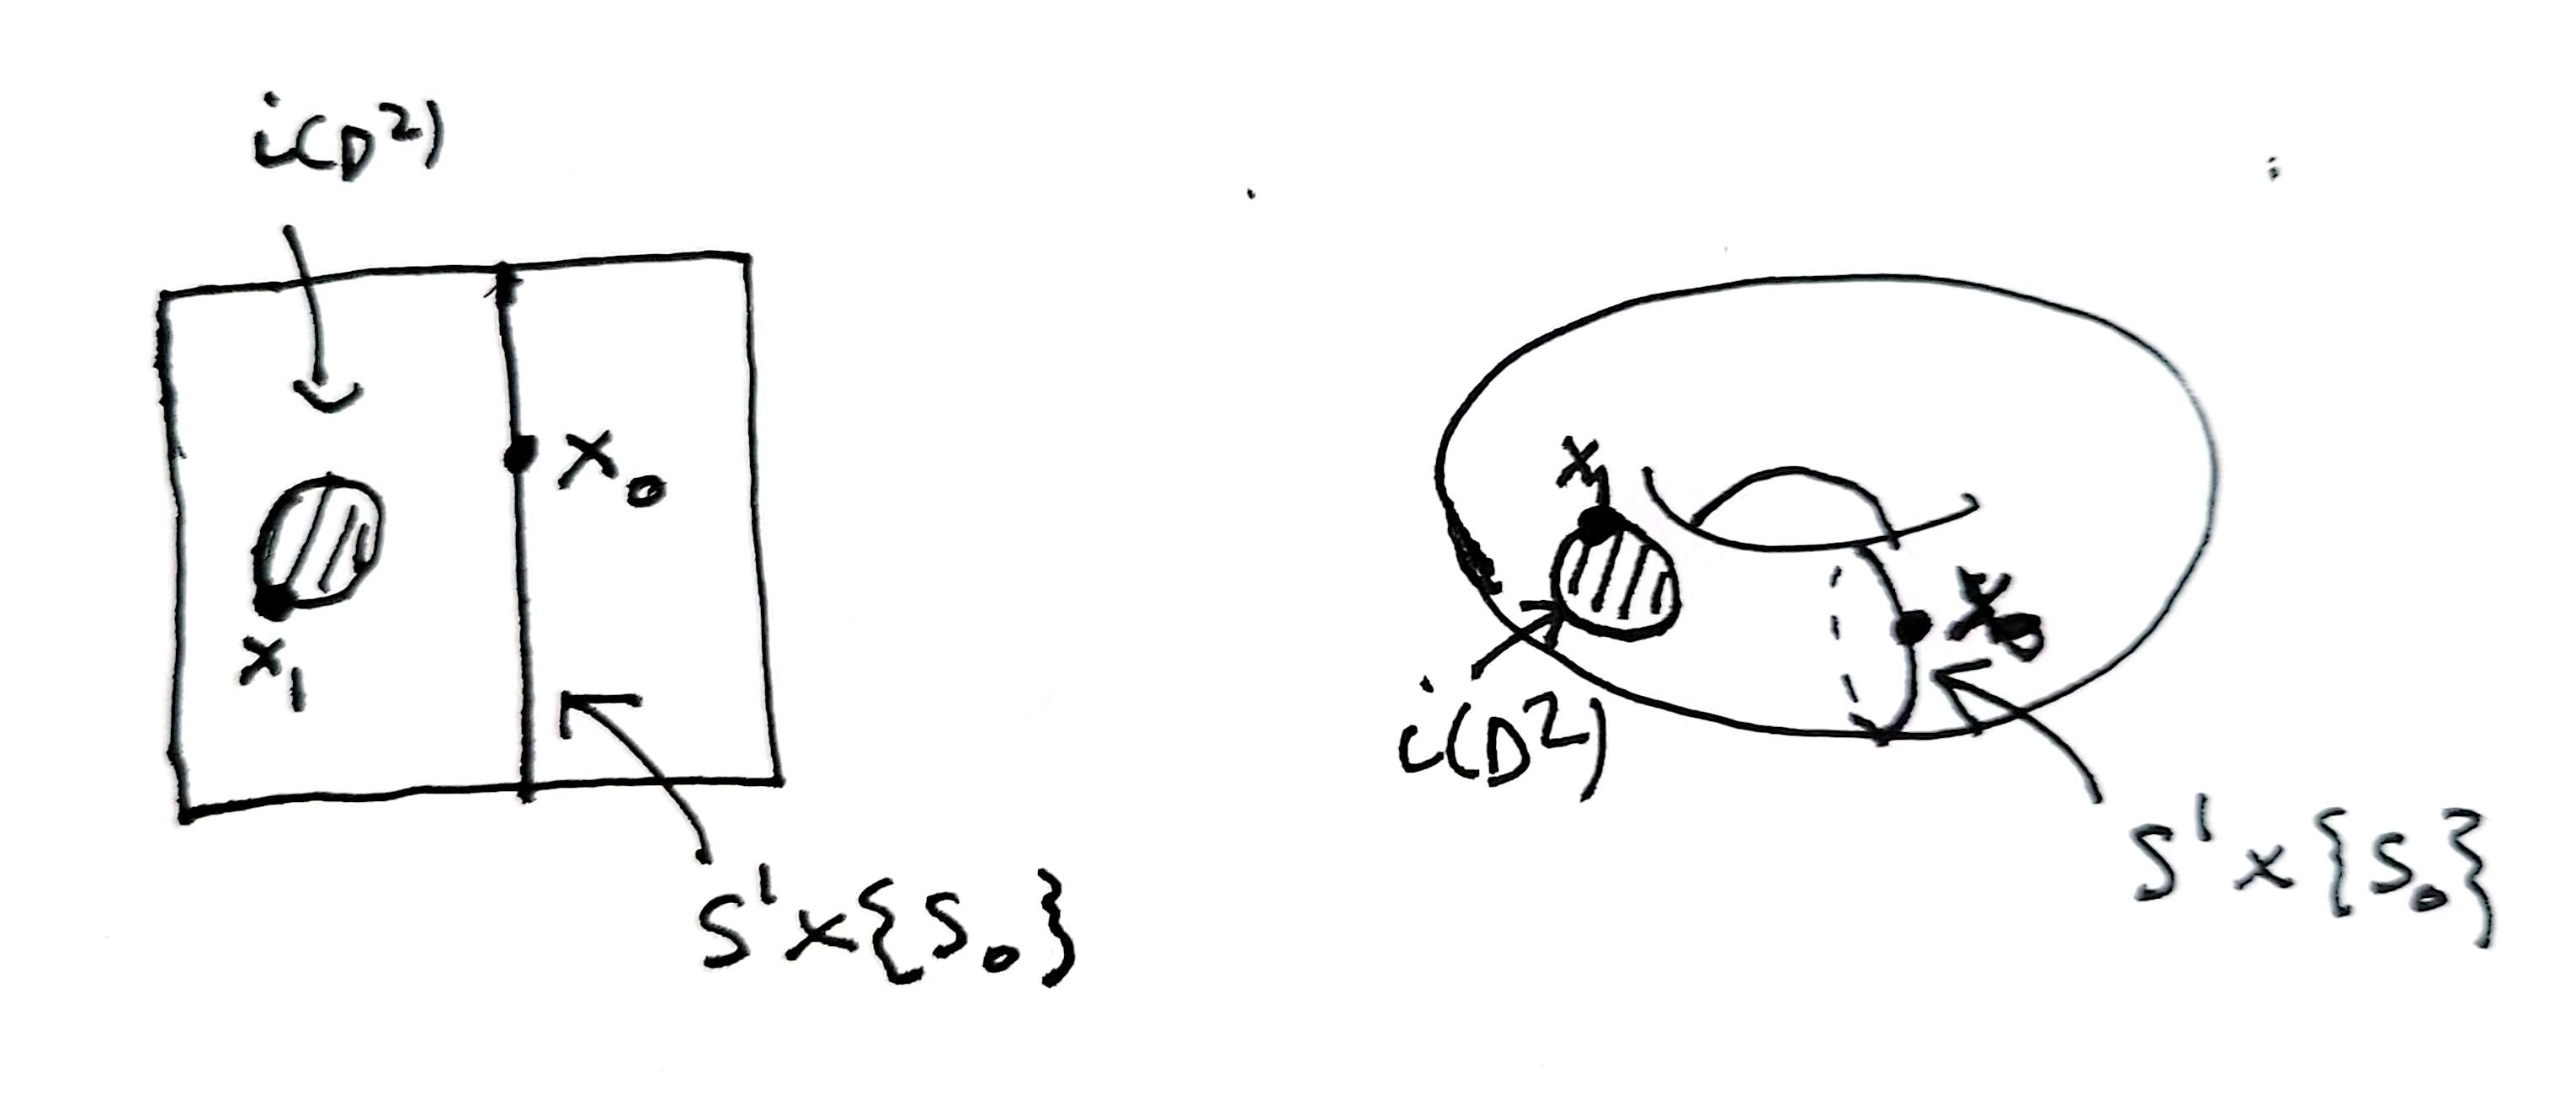
\includegraphics[width=0.8\textwidth]{p11.jpeg}
            \caption{Note that 
            in this figure, $A$ are the parts drawn
        without the interior of the disk $i(D^2)$.}
            \label{fig:p11-jpeg}
        \end{figure}

        (2)
        Recall that
        \[
        \pi_n (T,A,x_1) =
        \left[ I^{n},\partial I^{n},
        J^{n-1}; T,A, x_1 \right] .
        \] 
        Thus $\pi_1 \left( T,A,x_1 \right) $ becomes
        the set of homotopy classes
        of maps
        $\left( I, \left\{ 0,1 \right\} , \left\{ 1 \right\} 
        \right) \to \left( T,A,x_1 \right)$. That is, the
        set of paths in $T$ starting at a point in $A$ and
        ending at $x_1$.
        Now, take a path $\gamma$ from
        $x_1$ to $x_0$, and for
        a path $\left[ \alpha \right]  \in 
        \pi_1 \left( T,A,x_1 \right) $, we
        can homotopy this path to start at
        $x_0$, so by
        concatinating $\gamma$ with this path, we
        obtain a closed loop in $T \cong \mathbb{Z} \oplus \mathbb{Z}$,
        so to obtain a well-defined map, we homotopy $\alpha$ to
        the path in $\left[ \alpha \right] $ which, when
        we concatinate with $\gamma$, has
        $0$ in the second coordinate. That is,
        $\left[ \gamma * \alpha \right] =
        \left( n,0 \right) $ in
        $\pi_1 \left( T,x_1 \right) $. Denote this
        map $k \colon \pi_1 \left( T,A,x_1 \right) 
        \to \pi_1 \left( T,x_1 \right) $.
        The kernel of this map is all maps
        which, when concatenated with $\gamma$, become
        $\left( 0,0 \right) $ in
        $\pi_1 \left( T,x_1 \right) $. But $\gamma$ can
        be chosen to 


        We have
        \[
            \underbrace{\pi_1(A,x_1)}_{\mathbb{Z}} 
            \stackrel{0}{\to} 
        \underbrace{\pi_1 (T, x_1)}_{\mathbb{Z}^2} \to 
        \pi_1 \left( T,A,x_1 \right) 
        \to \underbrace{\pi_0 (A,x_1)}_{\cong \mathbb{Z}/2}
        \to \underbrace{\pi_0 (T,x_1)}_{1}
        \] 

        (3) Using the LES of relative homotopy groups, we
        have that
        \begin{align*}
            \pi_2 (T,x_i)
            \to \pi_2 \left( T,A, x_i \right) 
            \to \pi_1 \left( A,x_i \right) \to 
            \pi_1 \left( T,x_i \right) 
        \end{align*}
        is exact for $i = 0,1$.
        For $i=0,1$, 
        $\pi_1 (A,x_i) \cong \mathbb{Z}$ and
        $\pi_1 (T,x_i) \cong \mathbb{Z}^2$, while
        $\pi_2 \left( T,x_i \right) \cong 1$ for
        both $i=0,1$.
    \end{solution}


    \begin{problem}[]
        \begin{enumerate}
            \item Compute $\pi_1 \left( S^{1} \vee
                S^2\right) $ and describe the universal
                cover of $S^{1} \vee S^2$.
            \item Show that $\pi_2 \left( S^{1} \vee
                S^2 \right) $ is isomorphic
                to $\bigoplus_{\mathbb{Z}} \mathbb{Z}$.
            \item Explicitly describe the action of
                $\pi_1 \left( S^{1} \vee S^2 \right) $ on
                $\bigoplus_{\mathbb{Z}} \mathbb{Z} \cong
                \pi_2 \left( S^{1} \vee S^2 \right) $.
        \end{enumerate}
    \end{problem}

    \begin{solution}
        (1) From the LES, we have
        \[
            \underbrace{\pi_1 \left( S^2, * \right)}_{
            \cong 0} \to 
        \pi_1 \left( S^{1} \vee S^2, * \right) 
        \to 
        \underbrace{\pi_1 \left( S^{1} \vee S^2, S^2 , * \right)}_{
        \cong \mathbb{Z}}
        \to \underbrace{\pi_0 \left( S^2, * \right)}_{\cong 0}
        \] 
        so we find that
        $\pi_1 \left( S^{1} \vee S^2, * \right) 
        \cong \mathbb{Z}$.
        The universal cover of $S^{1} \vee S^2$ is
        easily seen to be
        $\mathbb{R}$ with a copy of $S^2$ attached to
        each integer of $\mathbb{R}$.\\
        (2) To compute
        $\pi_2 \left( S^{1} \vee S^2 \right) $, it suffices
        to compute $\pi_2$ of its universal cover since
        these are isomorphic. The universal cover
        is $\mathbb{R}$ with $S^2$ attached at each integer.
        Since $\mathbb{R} \simeq \left\{ * \right\}$, the
        universal cover is homotopy equivalent to
        $\vee_{\mathbb{Z}} S^2$.
        Consider the LES for the pair
        $\left( \prod_{\mathbb{Z}} S^2, 
        \vee_{\mathbb{Z}} S^2 \right) $ :
        \[
        \pi_{3} \left( \prod_{\mathbb{Z}} S^2, 
        \bigvee_{\mathbb{Z}} S^2\right) \to 
        \pi_2 \left( \bigvee_{\mathbb{Z}} S^2 \right)
        \to \pi_2 \left( \prod_{\mathbb{Z}} S^2 \right) 
        \to \pi_2 \left( \prod_{\mathbb{Z}} S^2,
        \bigvee_{\mathbb{Z}} S^2 \right) 
        \] 
        Now,
        $\pi_{2}\left( \prod_{\mathbb{Z}}S^2 \right) 
        \cong \oplus_{\mathbb{Z}} \pi_2 \left( S^2 \right) 
        \cong \oplus_{\mathbb{Z}} \mathbb{Z}$ (with
        the inclusions
        $S^2 \hookrightarrow \prod_{\mathbb{Z}}S^2$ 
        whose induced images form a basis, hence
        if $\pi_2 \left( \prod_{\mathbb{Z}} S^2 \right) 
        \cong \pi_2 \left( \bigvee_{\mathbb{Z}}S^2 \right) $ 
        under the inclusion
        $\bigvee_{\mathbb{Z}}S^2 \hookrightarrow 
        \prod_{\mathbb{Z}}S^2$, then
        the same basis also holds for
        $\pi_2 \left( \bigvee_{\mathbb{Z}}S^2 \right) $), since
        $\pi_k \left( \prod_{\alpha} X_\alpha \right) \cong
        \oplus_{\alpha} \pi_k \left( X_{\alpha} \right) $.
        We now claim that
        $\pi_n \left( 
        \prod_{\mathbb{Z}} S^2, 
    \bigvee_{\mathbb{Z}} S^2 \right) \cong 0$ for
    $n \le 3$. To this end,
    note that on p. 8 in Hatcher, it is described that
    we can give products $X \times Y$, we can give
    these a CW structure when $X$ and $Y$ have a CW structure,
    given by a cell complex with cells
    the products $e_{\alpha}^{m} \times 
    e_{\beta}^{n}$ for $e_{\alpha}^{m}$ ranging over
    the cells of $X$ and $e_{\beta}^{n}$ ranging over the
    cells of $Y$. Choosing
    $\left( s_0, s_0, \ldots, s_0 , \ldots \right) $ as
    a $0$-cell in $\prod_{\mathbb{Z}}S^2$ and
    attaching $2 $-cells to obtain
    $\bigvee_{\mathbb{Z}}S_i^2$ by
    $S_{i}^2$ identified with
    with the $i$ th coordinate copy of
    $S_i^2$ in $\prod_{i \in \mathbb{Z}}S_i^2$ (so all other
    coordinates or $s_0$ ).
    We then precisely find that
    $\bigvee_{\mathbb{Z}} S^2$ constitutes
    the $2$-skeleton for
    $\prod_{\mathbb{Z}}S^2$. By
    Corollary 4.12 in Hatcher, we then find that
    $\left( \prod_{\mathbb{Z}} S^2, 
    \bigvee_{\mathbb{Z}} S^2 \right) $ is
    $3$-connected. The result follows.\\
    (3) 



    \end{solution}


    \begin{problem}[]
        Let $\left( X,A,x_0 \right) $ be a pointed pair
        such that the inclusion
        $i \colon A \hookrightarrow X$ is based nullhomotopic
        (the nullhomotopy preserves the basepoint). The goal
        is to show that for $n\ge 2$, there is an isomorphism
        of groups:
        \[
        \pi_n (X,A,x_0) \cong \pi_n (X,x_0) \times 
        \pi_{n-1}(A,x_0).
        \] 
        \begin{enumerate}
            \item Show that there is an exact sequence
                of groups
                \[
                1 \to \pi_n (X,x_0) 
                \stackrel{j_*}{\to} 
                \pi_n \left( X, A, x_0 \right) 
                \stackrel{\partial_*}{\to} 
                \pi_{n-1}(A,x_0) \to 1.
                \] 
            \item Using a based nullhomotopy
                $H \colon A \times \left[ 0,1 \right] 
                \to X$, construct a natural group morphism
                \[
                r_* \colon \pi_n (X,A,x_0) \to 
                \pi_n (X,x_0)
                \] 
                such that $r_* \circ j_* = 1$.
            \item Show that for any short exact sequence
                of groups
                \[
                1 \to A \stackrel{\alpha}{\to} 
                B \stackrel{\beta}{\to} C \to 1
                \] 
                such that $\alpha$ admits a retraction, there
                is a group isomorphism
                \[
                B \cong A \times C.
                \] 
                Conclude the desired isomorphism.
        \end{enumerate}
    \end{problem}

    \begin{proof}
        (1) From the LES for relative homotopy groups, we obtain that
        \[
        \pi_n (A, x_0) \stackrel{i_*}{\to}  \pi_n(X,x_0)
        \stackrel{j_*}{\to} \pi_n \left( X, A, x_0 \right) 
        \stackrel{\partial_*}{\to} 
        \pi_{n-1}(A,x_0) \stackrel{i_*}{\to} 
        \pi_{n-1} \left( X, x_0 \right) 
        \] 
        is exact.
        For $n\ge 2$, all the sets in the exact sequence are
        groups and the maps are group homomorphisms.
        Since homotopic maps relative to the base point induce
        the same maps on homotopy groups, we find by assumption
        that $i_* = 0$. Therefore,
        \[
        1 \stackrel{0}{\to}   \pi_n(X,x_0)
        \stackrel{j_*}{\to} \pi_n \left( X, A, x_0 \right) 
        \stackrel{\partial_*}{\to} 
        \pi_{n-1}(A,x_0) \stackrel{0}{\to} 
        1
        \] 
        is exact.\\
        \linebreak
        (2) Let
        $\left[ f \right] \in \pi_n \left( X, A,x_0 \right) $.

    \end{proof}



    %\printbibliography
\end{document}
